\documentclass[xcolor={dvipsnames}]{beamer}
\mode<presentation>{\usetheme{boxes}}
\usecolortheme{default}
\setbeamertemplate{navigation symbols}{}%remove navigation symbols

\setbeamerfont{frametitle}{size=\Large}

%\setbeamercolor{structure}{fg=beamer@blendedblue}



\setbeamertemplate{bibliography item}{\insertbiblabel}

\setbeamercolor{bibliography entry author}{fg=black}
\setbeamercolor{bibliography entry title}{fg=black} 
\setbeamercolor{bibliography entry location}{fg=black} 
\setbeamercolor{bibliography entry note}{fg=black}  

\usepackage[style=numeric,sorting=ydnt,maxnames=1,defernumbers=true, firstinits=true]{biblatex}
\renewbibmacro{in:}{}
\ExecuteBibliographyOptions{sorting=ydnt}

%\addbibresource{./jlescSummerSchool_checkpointing.bib}

\makeatother
\setbeamertemplate{footline}
{
  \leavevmode%
  \hbox{%
    %% \begin{beamercolorbox}[wd=.2\paperwidth,ht=2.25ex,dp=1ex]{date in head/foot}%
    %%   \usebeamerfont{date in foot}
    %% \end{beamercolorbox}%
  %%   \begin{beamercolorbox}[wd=.6\paperwidth,ht=2.25ex,dp=1ex, center]{date in head/foot}%
  %%     \usebeamerfont{date in foot}\insertshortdate
  %% \end{beamercolorbox}%
  \begin{beamercolorbox}[wd=\paperwidth,ht=2.25ex,dp=1ex]{date in head/foot}%
    \usebeamerfont{date in foot}\hfill
    {\scriptsize\insertframenumber{}}\hspace*{2ex}
  \end{beamercolorbox}}%
  \vskip0pt%
}
\makeatletter



\usepackage[utf8]{inputenc}
%\usepackage[T1]{fontenc}
%\usepackage[francais]{babel}
\usepackage{hyperref}
\usepackage{url}
\usepackage{pifont}
\usepackage{changepage}
\usepackage{listings}
\lstset{basicstyle=\ttfamily,
  showstringspaces=false,
  commentstyle=\color{black},
  keywordstyle=\color{black}
}

\usepackage{fancyvrb}
\usepackage{multirow}
\usepackage{tabu} 
\usepackage{colortbl}

\usepackage{marvosym}

\usepackage{eurosym}

\usepackage{gitdags}
\usepackage{comment}

\usepackage{pdfpages}
\setbeamercolor{background canvas}{bg=}


\usepackage{perpage} %the perpage package
\MakePerPage{footnote}



\definecolor{beamer@blendedblue}{RGB}{0,102,204}

\definecolor{beamer@lightgray}{RGB}{238,238,224}


\definecolor{itemorange}{RGB}{255,114,0}


\definecolor{myorange}{RGB}{255,103,0}


\setbeamertemplate{itemize items}[circle]
\setbeamertemplate{itemize subitem}[triangle]


\setbeamercolor{itemize item}{fg=beamer@blendedblue}
\setbeamercolor{itemize subitem}{fg=gray}


\newcommand<>{\Blue}[1]{{\color#2{beamer@blendedblue}#1}}
%\newcommand<>{\Orange}[1]{{\color#2{BurntOrange}#1}}
\newcommand<>{\Orange}[1]{{\color#2{myorange}#1}}
\newcommand<>{\Alert}[1]{{\Orange{\textbf{#1}}}}


\newcommand{\largeskip}{\vspace{0.6cm}}
\newcommand{\hugeskip}{\vspace{1cm}}



\usepackage{tikz}
\usetikzlibrary{%
decorations.pathreplacing,%
decorations.pathmorphing,%
decorations.shapes,%
decorations.text,%
decorations.markings,%
shapes,%
shapes.callouts,%
shadows,%
arrows,
calc,%
positioning,%
chains,%
backgrounds,%
fit, %
fadings}






\tikzset{
    invisible/.style={opacity=0},
    visible on/.style={alt={#1{}{invisible}}},
    alt/.code args={<#1>#2#3}{%
      \alt<#1>{\pgfkeysalso{#2}}{\pgfkeysalso{#3}} % \pgfkeysalso doesn't change the path
    },
}


\tikzset{
    colornode/.style={
        outer sep=0pt, fill=#1!67, %text height=2ex, text depth=.5ex
    },
    cpu/.style={
        diamond, fill=gray!30, aspect=3, name=CPU#1,
        node contents={$\text{CPU}_{#1}$},
    },
    thread/.style={fill=#1!67,
        minimum width=5ex, minimum height=1.25em},
    tick/.style={very thin},
}



\newcommand{\email}[1]{\href{mailto:#1}{\nolinkurl{#1}}}

\newcommand{\xmark}{\ding{55}}


\AtBeginPart{
  %\frame{\partpage}
  \frame{
    \frametitle{Agenda}
    \small
    \tableofcontents[part=\insertpartnumber,
    sectionstyle=show,
    subsectionstyle=hide,
    subsubsectionstyle=hide]
  }
}

\AtBeginSection[]
{
  \begin{frame}
    \frametitle{Agenda}
    \small
    \tableofcontents[
    sectionstyle=show/shaded,
    subsectionstyle=show/show/hide,
    subsubsectionstyle=hide]
  \end{frame}
}

\AtBeginSubsection[]{
  \mode<presentation>{
    \frame{\tableofcontents[
      sectionstyle=show/hide,
      subsectionstyle=show/shaded/hide,
      subsubsectionstyle=show/show/hide]
    }
  }
}


\date[\the\year]{\the\year}

\newcommand{\shellcmd}[1]{\indent\indent\texttt{\footnotesize\$ #1}}


\title[]{Cloud Computing}
\subtitle{Mise à niveau Git\footnote{Adapté du cours DevOps de Thomas ROPARS (cf dernier slide)}}

%Thomas ROPARS : \url{https://tropars.github.io/teaching/},
%\url{https://roparst.gricad-pages.univ-grenoble-alpes.fr/cloud-tutorials/m2gi-devops/}}}


\author[]{\\Danilo Carastan dos Santos
  \\ \vspace{0.5cm} \email{danilo.carastan-dos-santos@univ-grenoble-alpes.fr}}

\definecolor{mybrown}{RGB}{205,133,63}
\definecolor{myblue}{RGB}{28,134,238}

\let\Red=\alert
\newcommand<>{\green}[1]{{\color#2{green!70!black}#1}}
\newcommand<>{\blue}[1]{{\color#2{blue!100!black!100}#1}}
\definecolor{darkgreen}{rgb}{0,0.5,0}

\newcommand\myvdots{{\smash[b]\strut\smash[t]\vdots}}


\usepackage{boxedminipage}
\newenvironment{boitecode}[1]{
    \begin{boxedminipage}{\linewidth}      
%\begin{beamerboxesrounded}[shadow=true,lower=lightex,upper=medex]{#1}
    #1
    \begin{semiverbatim}
}{   \end{semiverbatim}\vspace{-1.5\baselineskip}
    \end{boxedminipage}
%  \end{beamerboxesrounded}
}


\begin{document}


\begingroup
\setbeamercolor{titlelike}{bg=beamer@lightgray, fg=black}
\begin{frame}
\titlepage
\end{frame}

\endgroup

\begin{frame}{Motivations}

  \begin{center}
    \Large{Une équipe de développeurs participe à la réalisation d'une
    application.}
  \end{center}

  \smallskip
  Pour pouvoir être efficace dans votre nouvel environnement, il vous
  faudra:
  \begin{itemize}
  \item Comment conserver un historique ?
  \item Comment revenir en arrière ?
  \item Comment travailler à plusieurs en parallèle sur le même code ?
  \item Comment gérer plusieurs versions du code à la fois ?
  \item Comment savoir ce qui a été modifié et par qui (et pourquoi)?
  \end{itemize}

  \begin{center}
    \Large{\Alert{Solution : utiliser un VCS (\textit{Version Control Software})}}
  \end{center}
  
\end{frame}

\begin{frame}{Ce qu'on y stocke}

    \textbf{Ce qu'on y met}    
    \begin{itemize}
        \item Fichiers source (.java, .c, .html. etc.)
        \item Fichiers binaires non dérivés des sources (images, pdfs non générés
        par code source)
        \item Fichiers de configuration, compilation (Makefile, .yaml, etc)
    \end{itemize}

    \pause
    \bigskip

    \Alert{Ce qu'on n'y met pas}
    \begin{itemize}
        \item Fichiers temporaires (.log, .out, etc)
        \item Fichiers générés (.jar, .class, .o, .exe, .pdf)
    \end{itemize}
    
\end{frame}

\begin{comment}

\begin{frame}{Avant de commencer \ldots}

    \begin{block}{Warning}
  
      Remarque introductive, présentation de GIT @ Google par Linus
      Torvalds, 2007.
    
      \begin{quote}
  
      [Linus] is a guy who delights being cruel to people.
      His latest cruel act is to create a revision control
      system which is expressly designed to make you
      feel less intelligent than you thought you were.
      [\ldots] So Linus is here today to explain to us why on
      earth he wrote a software tool which, eh, only he is
      smart enough to know how to use.
      
      \end{quote}
    \end{block}
  
    \bigskip
    
    Git est un outil très puissant. Il nous permet aussi de faire de très
    grosses bêtises.
    
  \end{frame}

\end{comment}

  \begin{frame}{L’essentiel : Commit}
    Un Commit stocke l’état d’une partie du dépôt à un instant donné. 

    Quelques informations importantes stockées dans un commit :
    
    \begin{itemize}
        \item Un pointeur vers un ou plusieurs autres Commits (historique)
        \item Les informations sur l’auteur du Commit
        \item Une description sous forme d’une chaîne de caractères
    \end{itemize}

  \end{frame}

\begin{frame}{Les commandes}

  Git est un ensemble de commandes. Les commandes sont de la forme:
  \medskip
  \begin{center}
    \texttt{\large git commande options}
  \end{center}

  \bigskip
  \begin{block}{Exemple}
  \medskip
  \begin{center}
    \texttt{\large git add file1.txt}
  \end{center}
  \end{block}

  
\end{frame}

\begin{frame}[fragile]
  \frametitle{Création d'un dépôt}
  
  \begin{block}{Création d'un dépôt \emph{serveur}}
    \small{
\begin{verbatim}
$ mkdir projet.git
$ cd projet.git
$ git --bare init
\end{verbatim}}
  \end{block}

    \bigskip

    \begin{itemize}
    %% \item Pas de répertoire \texttt{xxx/.git} mais directement un \texttt{xxx.git/}
    \item Ne contient pas les fichiers versionnés, mais juste
      l'historique
    \item On ne travaille pas sur cette version
    \end{itemize}

  
\end{frame}


\begin{frame}[fragile]
  \frametitle{Création d'un dépôt}

  \begin{block}{Initialisation d'un dépôt}
    \small{
\begin{verbatim}
$ cd myproject
$ git init
$ git add .
$ git commit -m 'initial commit'
$ git remote add origin git@gitserver:/XX/XX/project.git
$ git push origin master
\end{verbatim}}
  \end{block}
  
  \bigskip

    \begin{itemize}
    \item Créer un répertoire local \texttt{myproject} pour stocker
      notre version du projet.
    \item Associer le dépôt local avec le dépôt distant
    \item Envoyer l'état initial du dépôt vers le serveur
    \item À partir de ce moment, tout le monde peut obtenir sa copie
      locale du dépôt en utilisant \texttt{git clone}
    \end{itemize}
  

  
\end{frame}

\begin{frame}[fragile]
  \frametitle{Cloner un dépôt existant}

  Très souvent, un dépôt existe déjà. On veut alors récupérer une
  copie de ce dépôt.

  \medskip
  \begin{block}{Cloner un dépôt}
      \small{
\begin{verbatim}
$ git clone URL
\end{verbatim}}
    
  \end{block}

  \bigskip
  \begin{itemize}
  \item Crée une copie locale du dépôt entier.
  \item L'URL peut être de la forme :
    \begin{itemize}
    \item file://./myproject/project.git
    \item
      http://git.kernel.org/pub/scm/linux/kernel/git/torvalds/linux-2.6.git
    \item git://github.com/schacon/grit.git
    \end{itemize}
  \end{itemize}
  
\end{frame}

\begin{frame}[fragile]
    \frametitle{Quelques commandes}
  
    \begin{description}
    \item[\texttt{add}] : Ajoute dans l’\Blue{index} un fichier à commiter dans son
      état actuel.
    \item[\texttt{commit}] : enregistre dans le dépôt local les modifications qui
  ont été ajoutées dans l’\Blue{index} par une commande add
    \item[\texttt{restore --staged}] : supprime la référence d’un fichier de
      l’\Blue{index} ajouté par une commande add.
    \end{description}
    \medskip
    L'index est aussi appelé \Blue{staging area}.
    \bigskip
  
    Souvent on veut simplement commiter toutes les modifications en
    cours (= fichiers de l'index + fichiers modifiés):
    \small{
  \begin{verbatim}
  $ git commit -a
  \end{verbatim}
      }  
  
\end{frame}

\begin{frame}[fragile]{Question}

    Supposons la structure du dossier suivant. Les fichiers \texttt{1-git.XX}
    sont générés par la compilation du fichier \texttt{1-git.tex}

    \begin{tiny} 
    \begin{center} 
    \begin{verbatim}
    $ 2024-2025-MIAGE/Cours/1-git$ ls -lah
    total 608K
    drwxrwxr-x 3 dancarastan dancarastan 4,0K juil.  5 16:36 .
    drwxrwxr-x 4 dancarastan dancarastan 4,0K juil.  5 10:06 ..
    -rw-rw-r-- 1 dancarastan dancarastan 2,5K juil.  5 16:36 1-git.aux
    -rw-rw-r-- 1 dancarastan dancarastan    0 juil.  5 10:47 1-git.bbl
    -rw-rw-r-- 1 dancarastan dancarastan 104K juil.  5 16:36 1-git.bcf
    -rw-rw-r-- 1 dancarastan dancarastan  41K juil.  5 16:36 1-git.fdb-latexmk
    -rw-rw-r-- 1 dancarastan dancarastan 130K juil.  5 16:36 1-git.fls
    -rw-rw-r-- 1 dancarastan dancarastan  67K juil.  5 16:36 1-git.log
    -rw-rw-r-- 1 dancarastan dancarastan 1,2K juil.  5 16:36 1-git.nav
    -rw-rw-r-- 1 dancarastan dancarastan    0 juil.  5 16:36 1-git.out
    -rw-rw-r-- 1 dancarastan dancarastan 178K juil.  5 16:36 1-git.pdf
    -rw-rw-r-- 1 dancarastan dancarastan 2,2K juil.  5 16:36 1-git.run.xml
    -rw-rw-r-- 1 dancarastan dancarastan    0 juil.  5 16:36 1-git.snm
    -rw-rw-r-- 1 dancarastan dancarastan  23K juil.  5 16:36 1-git.synctex.gz
    -rw-rw-r-- 1 dancarastan dancarastan  13K juil.  5 16:36 1-git.tex
    -rw-rw-r-- 1 dancarastan dancarastan    0 juil.  5 16:36 1-git.toc
    -rw-rw-r-- 1 dancarastan dancarastan  608 juil.  5 16:36 1-git.vrb
    drwxrwxr-x 2 dancarastan dancarastan 4,0K juil.  5 10:40 Figures
    -rw-rw-r-- 1 dancarastan dancarastan 7,3K juil.  5 10:45 gitdags.sty
    -rw-rw-r-- 1 dancarastan dancarastan  273 juil.  5 10:06 Makefile
    \end{verbatim}
    \end{center}
    \end{tiny}
        
    Je décide d'utiliser \texttt{git add .} et puis \texttt{git commit -m "My
    commit"}. Que se passera-t-il ?
\end{frame}

\begin{frame}[fragile]{Réponse}

    \textbf{Réponse 1 : } Il ne se passera rien, le dépôt n'est pas initialisé. On
    devrait initialiser le dépôt avec
    
    \begin{verbatim}
    $ git init .
    \end{verbatim}

    \textbf{Réponse 2 : } Supposons que le dépôt est déjà initialisé, tous les
    fichiers temporaires (.aux, .log, etc) et pdf générés par la compilation
    \LaTeX (1-git.pdf) seront commités. 

    \textbf{Solutions : } 
    \begin{description}
        \item[pénible :] Ajouter (\texttt{git add}) chaque fichier
        individuellement
        \item[recommandé :] Utiliser un fichier
        \texttt{.gitignore}\footnote{\href{https://git-scm.com/book/fr/v2/Les-bases-de-Git-Enregistrer-des-modifications-dans-le-d\%C3\%A9p\%C3\%B4t}{https://git-scm.com/book/fr/v2/Les-bases-de-Git-Enregistrer-des-modifications-dans-le-dépôt}.
        Partie ``Ignorer des fichiers''}
    \end{description}
     
   
        
    
\end{frame}


\begin{frame}{Le cycle de vie d'un fichier}

  \begin{center}
    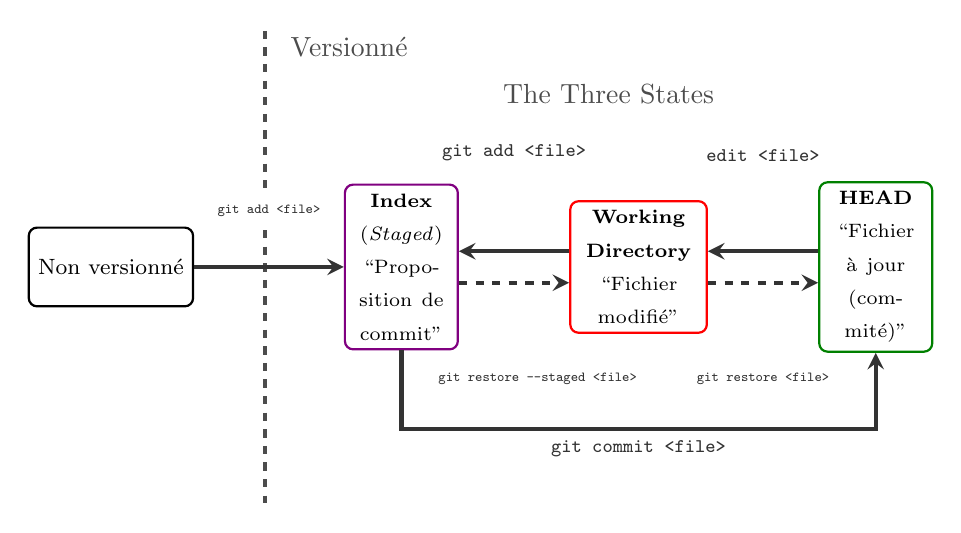
\begin{tikzpicture}

      \node(nv) [draw=black,minimum height=1cm, rounded corners=3pt,thick] {\footnotesize Non versionné};

      \node(staged) at ($(nv.east)+(1.9,0)$) [draw=violet,minimum
        height=1cm, text
        width=1.2cm, align=center, rounded corners=3pt,thick, anchor=west] {\scriptsize \Blue{\textbf{Index}} (\emph{Staged}) ``Proposition de commit''};

      \node(modified) at ($(staged.east)+(1.4,0)$) [draw=red,minimum
        height=1cm, align=center, rounded corners=3pt,thick, anchor=west, text width=1.5cm] {\scriptsize \Blue{\textbf{Working Directory}} ``Fichier modifié''};

      \node(uptodate) at ($(modified.east)+(1.4,0)$) [draw=darkgreen,minimum
        height=1cm, align=center, rounded corners=3pt,thick, anchor=west, text width=1.2cm] {\scriptsize \Blue{\textbf{HEAD}} ``Fichier à jour (commité)''};


      %vertical limit

      \draw[dashed, very thick,black!70] ($(nv.east)+(0.9,3)$) --
      +(0,-6);

      \node at ($(nv.east)+(1.1,2.8)$) [anchor=west,black!70] {Versionné};

      \node at ($(nv.east)+(3.8,2.2)$) [anchor=west,black!70] {The Three States};


      %arrows

      \draw[-stealth,black!80,ultra thick,visible on=<2->] (nv.east) -- node[above=0.5cm,fill=white,]
           {\texttt{\tiny{git add <file>}}}($(staged.west)+(0.0,0)$);

      \draw[-stealth,black!80,ultra thick,visible on=<5->] ($(modified.west)+(0,0.2)$) -- node[above=1cm]
           {\texttt{\scriptsize{git add <file>}}}($(staged.east)+(0,0.2)$);

      \draw[-stealth,black!80,ultra thick, visible on=<4->] ($(uptodate.west)+(0,0.2)$) -- node[above=1cm]
           {\texttt{\scriptsize{edit <file>}}} ($(modified.east)+(0,0.2)$);

      \draw[-stealth,black!80,ultra thick, visible on=<3->] (staged.south) -- +(0,-1) -|
      node[below,pos=0.25] {\texttt{\scriptsize{git commit <file>}}}(uptodate.south);

      \draw[-stealth,black!80,ultra thick, dashed, visible on=<6->] ($(staged.east)+(0,-0.2)$) -- node[below=1cm, xshift=0.3cm]
           {\texttt{\tiny{git restore --staged <file>}}}($(modified.west)+(0,-0.2)$);

      \draw[-stealth,black!80,ultra thick, dashed, visible on=<6->] ($(modified.east)+(0,-0.2)$) -- node[below=1cm]
           {\texttt{\tiny{git restore <file>}}}($(uptodate.west)+(0,-0.2)$);


      
      
    \end{tikzpicture}
  \end{center}

\end{frame}

\begin{frame}{La notion d'historique}

  %\textbf{Historique de changements :} L’historique est un graphe orienté composé d’un
  %ensemble de versions pouvant être recalculées à partir des versions adjacentes
  %en appliquant les \textit{patchs}. 

  \begin{itemize}
    \item Un \Blue{commmit} enregistre les modifications indexées (par une
    commande add) à un instant donné
    \item Une \Blue{branche} est un pointeur sur un commit
    \item Chaque commit pointe vers son prédécesseur
    \item La variable \Blue{HEAD} pointe sur la branche sur laquelle
      on travaille actuellement.
  \end{itemize}


  %\vspace{.5cm}

  \begin{center}

      \begin{tikzpicture}

          \gitDAG[grow right sep = 2em]{
            A -- B -- { 
              C , 
                D -- E ,
              } -- F,
            };
          \gitbranch
            {master}      % node name and text 
            {above=of F} % node placement
            {F}
          \gitHEAD
            {above=of master} % node placement
            {master}          % target
          \gitbranch
            {maBranche}      % node name and text 
            {above=of E, yshift=0.7cm} % node placement
            {E} 
      
        \end{tikzpicture}        

  \end{center}
  
\end{frame}

\begin{frame}[fragile]{Historique : les branches}

\begin{itemize}
  \item L'historique peut inclure plusieurs \Blue{branches}, c'est-à-dire des
  sous-graphes qui évoluent en parallèle.
\end{itemize}


\vspace{0.8cm}

\begin{columns}
  
\begin{column}{.5\linewidth}
  \only<1>{
\begin{tikzpicture}

  \gitDAG[grow right sep = 2em]{
      A -- B ,
    };
    \gitbranch
        {master}      % node name and text 
        {above=of B} % node placement
        {B}
    \gitHEAD
        {above=of master} % node placement
        {master} 

\end{tikzpicture}
  }
  \only<2->{
  \begin{tikzpicture}
    \gitDAG[grow right sep = 2em]{
        {[nodes=highlighted node] A -- B } -- { 
          C,
          {[nodes=highlighted node] D -- E },
        }
      };
      \gitbranch
          {master}      % node name and text 
          {above=of C} % node placement
          {C}
      \gitbranch
          {maBranche}      % node name and text 
          {above=of E} % node placement
          {E}
      \gitHEAD
          {above=of maBranche} % node placement
          {maBranche}    
  \end{tikzpicture}
  }
\end{column}

\begin{column}{.55\linewidth}
  \begin{scriptsize}
    \begin{lstlisting}[language=bash]
      echo modif A > fichier1.txt      
      git add fichier1.txt
      git commit -m "commit A"
      echo modif B > fichier1.txt
      git commit -am "commit B"
    \end{lstlisting}
    \pause
    \vspace{-0.4cm}
    \begin{lstlisting}[language=bash]
      git branch maBranche
      echo modif C > fichier1.txt
      git commit -am "commit C"
      git checkout maBranche      
      echo modif D > fichier2.txt  
      git add fichier2.txt    
      git commit -m "commit D" 
      echo modif E > fichier2.txt
      git commit -am "commit E"      
    \end{lstlisting}
  \end{scriptsize}
  
\end{column}  

\end{columns}

%\begin{columns}
%  \begin{column}{.5\linewidth}
%    
%  \end{column}
%  
%  \begin{column}{.5\linewidth}
%    
%  \end{column}  
%  
%\end{columns}
 


\end{frame}
  

\begin{frame}[fragile]{Historique : les merges}

  On appelle \Blue{merge} toute version ayant un degré sortant strictement
  supérieur à 1. Cette version correspond alors à la fusion des \Blue{commits}
  de plusieurs branches.

  \vspace{.7cm}


  \begin{columns}
    \begin{column}{.5\linewidth}

      \only<1>{
        \begin{tikzpicture}
      
          \gitDAG[grow right sep = 1em]{
            A -- B -- { 
              C , 
                D -- E ,
              },       
            };
            \gitbranch
              {master}      % node name and text 
              {above=of C} % node placement
              {C}
            \gitbranch
              {maBranche}      % node name and text 
              {above=of E} % node placement
              {E}
            \gitHEAD
            {above=of maBranche} % node placement
            {maBranche} 
      
        \end{tikzpicture}
          }
      
          \only<2->{
        \begin{tikzpicture}
      
          \gitDAG[grow right sep = 1em]{
            A -- B -- { 
              C , 
                D -- E ,
              } -- {[nodes=highlighted node] F},
            };
            \gitbranch
              {master}      % node name and text 
              {above=of F} % node placement
              {F}
            % Add a branch node with adjusted height      
            \gitbranch        
              {maBranche}      % node name and text 
              {above=of E, yshift=0.55cm} % node placement
              {E}
            \gitHEAD
              {above=of master} % node placement
              {master} 
      
        \end{tikzpicture}
          }      
      
    \end{column}
    
    \begin{column}{.55\linewidth}
      \begin{scriptsize}    
    \pause
    \vspace{-0.4cm}
    \begin{lstlisting}[language=bash]
      git checkout master
      git merge maBranche      
    \end{lstlisting}
  \end{scriptsize}
    \end{column}  
    
  \end{columns}
\end{frame}

\begin{frame}[fragile]{Historique : les rebases}

  \begin{itemize}    
    \item Autre manière de fusionner 2 branches
    \item Fusionne entièrement la branche source dans la branche
      destination
    \item Permet de simplifier l'historique    
    \only<2>{
    \item \Alert{Ne jamais \emph{rebaser} des commits qui ont déjà été
      poussés sur un dépôt public}
      }
    \end{itemize}
    \only<3->{
    \begin{description}
      \item[fast-forward merge] lorsque le commit de destination est accessible
      en suivant l'historique des commits 
    \end{description}  
    }
  \vspace{.7cm}

\begin{columns}
  \begin{column}{.5\linewidth}
    \only<1>{
      \begin{tikzpicture}
    
        \gitDAG[grow right sep = 1em]{
          A -- B -- { 
            C, 
              D -- E ,
            }
          };
          \gitbranch
            {master}      % node name and text 
            {above=of C} % node placement
            {C}
          \gitbranch
            {maBranche}      % node name and text 
            {above=of E} % node placement
            {E}
          \gitHEAD
            {above=of master} % node placement
            {master}  
    
      \end{tikzpicture}
        }
    
        \only<2>{
      \begin{tikzpicture}
    
        \gitDAG[grow right sep = 1em]{
          A -- B -- { 
            C -- D -- E,        
            } 
          };
          \gitbranch
            {master}      % node name and text 
            {above=of C} % node placement
            {C}
          \gitbranch
            {maBranche}      % node name and text 
            {above=of E} % node placement
            {E}
          \gitHEAD
            {above=of maBranche} % node placement
            {maBranche}  
      \end{tikzpicture}
        }
      \only<3->{
      \begin{tikzpicture}
    
        \gitDAG[grow right sep = 1em]{
          A -- B -- { 
            C -- D -- E,        
            } 
          };
          \gitbranch
            {master}      % node name and text 
            {below=of E} % node placement
            {E}
          \gitbranch
            {maBranche}      % node name and text 
            {above=of E} % node placement
            {E}
          \gitHEAD
            {below=of master} % node placement
            {master}  
      \end{tikzpicture}     

        }

        
  \end{column}
  
  \begin{column}{.55\linewidth}
    \begin{scriptsize}    
      \pause      
      \begin{lstlisting}[language=bash]
        git checkout maBranche
        git rebase master      
      \end{lstlisting}
      \pause
      \vspace{-0.4cm}
      \begin{lstlisting}[language=bash]
        git checkout master
        git merge maBranche      
      \end{lstlisting}
    \end{scriptsize}    
  \end{column}  
 
\end{columns}
\end{frame}

\begin{frame}[fragile]{Revenir en arrière\footnote{Plus d'infos : \url{https://git-scm.com/book/fr/v2/Les-bases-de-Git-Annuler-des-actions}}}

  \Blue{Cas de modifications non commitées}

  \vspace{1.5cm}

    \begin{center}
      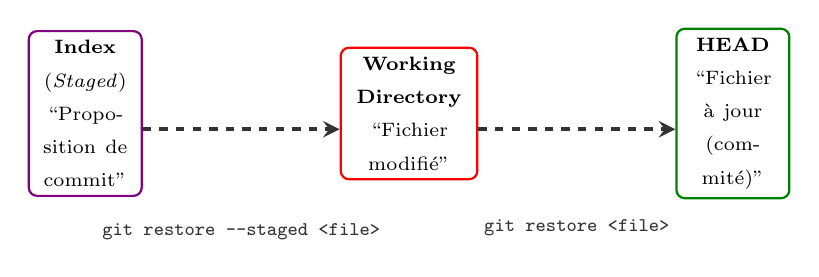
\begin{tikzpicture}
        
  
        \node(staged) at ($(0,0)$) [draw=violet,minimum
          height=1cm, text
          width=1.2cm, align=center, rounded corners=3pt,thick, anchor=west] {\scriptsize \Blue{\textbf{Index}} (\emph{Staged}) ``Proposition de commit''};
  
        \node(modified) at ($(staged.east)+(2.5,0)$) [draw=red,minimum
          height=1cm, align=center, rounded corners=3pt,thick, anchor=west, text width=1.5cm] {\scriptsize \Blue{\textbf{Working Directory}} ``Fichier modifié''};
  
        \node(uptodate) at ($(modified.east)+(2.5,0)$) [draw=darkgreen,minimum
          height=1cm, align=center, rounded corners=3pt,thick, anchor=west, text width=1.2cm] {\scriptsize \Blue{\textbf{HEAD}} ``Fichier à jour (commité)''};
  
  
        %arrows
  
        \draw[-stealth,black!80,ultra thick, dashed] ($(staged.east)+(0,-0.2)$) -- node[below=1.05cm, xshift=0.0cm]
             {\texttt{\scriptsize{git restore --staged <file>}}}($(modified.west)+(0,-0.2)$);
  
        \draw[-stealth,black!80,ultra thick, dashed] ($(modified.east)+(0,-0.2)$) -- node[below=1cm, xshift=0.0cm]
             {\texttt{\scriptsize{git restore <file>}}}($(uptodate.west)+(0,-0.2)$);
  
  
      \end{tikzpicture}
    \end{center}
  
\end{frame}

\begin{frame}{A propos de git checkout}

  \begin{block}{Une commande qui peut prêter à confusion}
    \begin{itemize}
    \item Permet de naviguer dans les branches
    \item Permet de modifier le contenu de fichiers
    \end{itemize}
  \end{block}

  \bigskip
  
  \begin{block}{Nouvelles commandes depuis git 2.23}
    \begin{itemize}
    \item \Blue{git switch} pour changer de branche
    \item \Blue{git restore} pour modifier le contenu d'un ficher
    \item A utiliser en remplacement de \texttt{git checkout}
    \end{itemize}
  \end{block}


  
\end{frame}


\begin{frame}[fragile]
  {Revenir en arrière}

  \begin{block}{Cas de modifications commitées}
    Trois commandes disponibles:
    \begin{description}
    \item[amend]: modifier le dernier commit
      \begin{itemize}
      \item Ajoute des fichiers au commit
      \item Changer le message de commit
      \end{itemize}
    \item[revert]: annuler un commit par un autre commit
    \item[reset]: rétablir la situation d'un ancien commit
    \end{description}
  \end{block}

  \largeskip
  \Alert{Si l'erreur a été rendue publique, la seule bonne pratique
    est \texttt{revert}.}
  
\end{frame}

\begin{frame}[fragile]{La commande reset\footnote{Plus d'infos : \href{https://git-scm.com/book/fr/v2/Utilitaires-Git-Reset-d\%C3\%A9mystifi\%C3\%A9}{https://git-scm.com/book/fr/v2/Utilitaires-Git-Reset-démystifié}}}
  
  \begin{itemize}
  %\item Annuler des ajouts dans l'index
  %  \small{
%\begin{verbatim}
%    git reset monfichier
%\end{verbatim}
%    }
%    \medskip
  \item Restaurer un ancien commit (mais en conservant toutes les
    modifications dans le \Blue{Working Directory} et \Blue{l'Index})
    \small{
\begin{verbatim}
    git reset --soft commitID
\end{verbatim}
    }
    \medskip
  \item Restaurer un ancien commit  et \Blue{l'Index} (mais en conservant toutes les
    modifications \Blue{Working Directory})
    \small{
\begin{verbatim}
    git reset commitID
\end{verbatim}
    }
    \medskip
  \item Restaurer un ancien commit, \Blue{l'Index}, et le \Blue{Working Directory}    
    \small{
\begin{verbatim}
    git reset --hard commitID
\end{verbatim}
    }
  \end{itemize}

\medskip
\Alert{Question : } quelle est la commande qui restaure le contenu des fichiers correspondants ?

\end{frame}

\begin{frame}{Pour aller plus loin}
  \begin{description}
    \item[Pro Git book] \url{https://git-scm.com/book/fr/v2}
    \item[GitHub Git Cheat Sheet] \url{https://education.github.com/git-cheat-sheet-education.pdf} 
    \item[Cours DevOps de Thomas ROPARS] \url{https://tropars.github.io/teaching/\#devops} 
  \end{description}
\end{frame}

\end{document}